
\chaptertoc{}

\addsec{Introduction}
\subimport{.}{introduction.tex}

\section{Généralités sur XXX}
\label{sec:9-1}
\subimport{Section1/}{section.tex}

\section{Grand Veymont}
\label{sec:9-2}
\subimport{Section2/}{section.tex}

%%
\section{Moucherotte}
\label{sec:9-3}
\subimport{Section3/}{section.tex}

\section{Modélisation du \emph{fil rouge}}
\label{sec:9-4}

La dernière alerte modélisée est le cas dit du \enquote{fil rouge} que
nous avions présenté dans le premier chapitre de cette thèse. Comme
nous l'avions indiqué lors de sa première présentation, le \emph{fil
  rouge} est une alerte particulière, contenant de nombreux indices
très imprécis et incertains. Par conséquent la \ac{zir} est
extrêmement étendue.


\subsection{Présentation de l'alerte}
\label{subsec:9-4-1}

Le fil rouge est une alerte composée de XX \emph{indices de
  localisation.}


Faute d'enregistrement audio, le fil rouge n'a pas été retranscrit,
les indices dont nous disposons (et qui avaient été présentés dans le
\autoref{chap:01}) ont donc été directement saisis par le secouriste.
%
de ce fait, le \emph{fil rouge} est une alerte assez différente des
précédentes, puisque XXX n'est pas
%
Le traitement du \emph{fil rouge} est donc plus proche du traitement
opérationnel qui sera réellement effectué lors du traitement d'une
alerte.



\subsection{Modélisation de l'alerte}
\label{subsec:9-4-2}

La \ac{zir} définie pour cette alerte est une zone de
\SI{625}{\kilo\meter\squared}

\begin{figure}
  \centering
  \begin{tikzpicture}
  \tikzset{et/.style={above,font=\footnotesize\vphantom{Ag}}}
  % 
  \node[inner sep=0pt, anchor=south west] (image) at (0,0){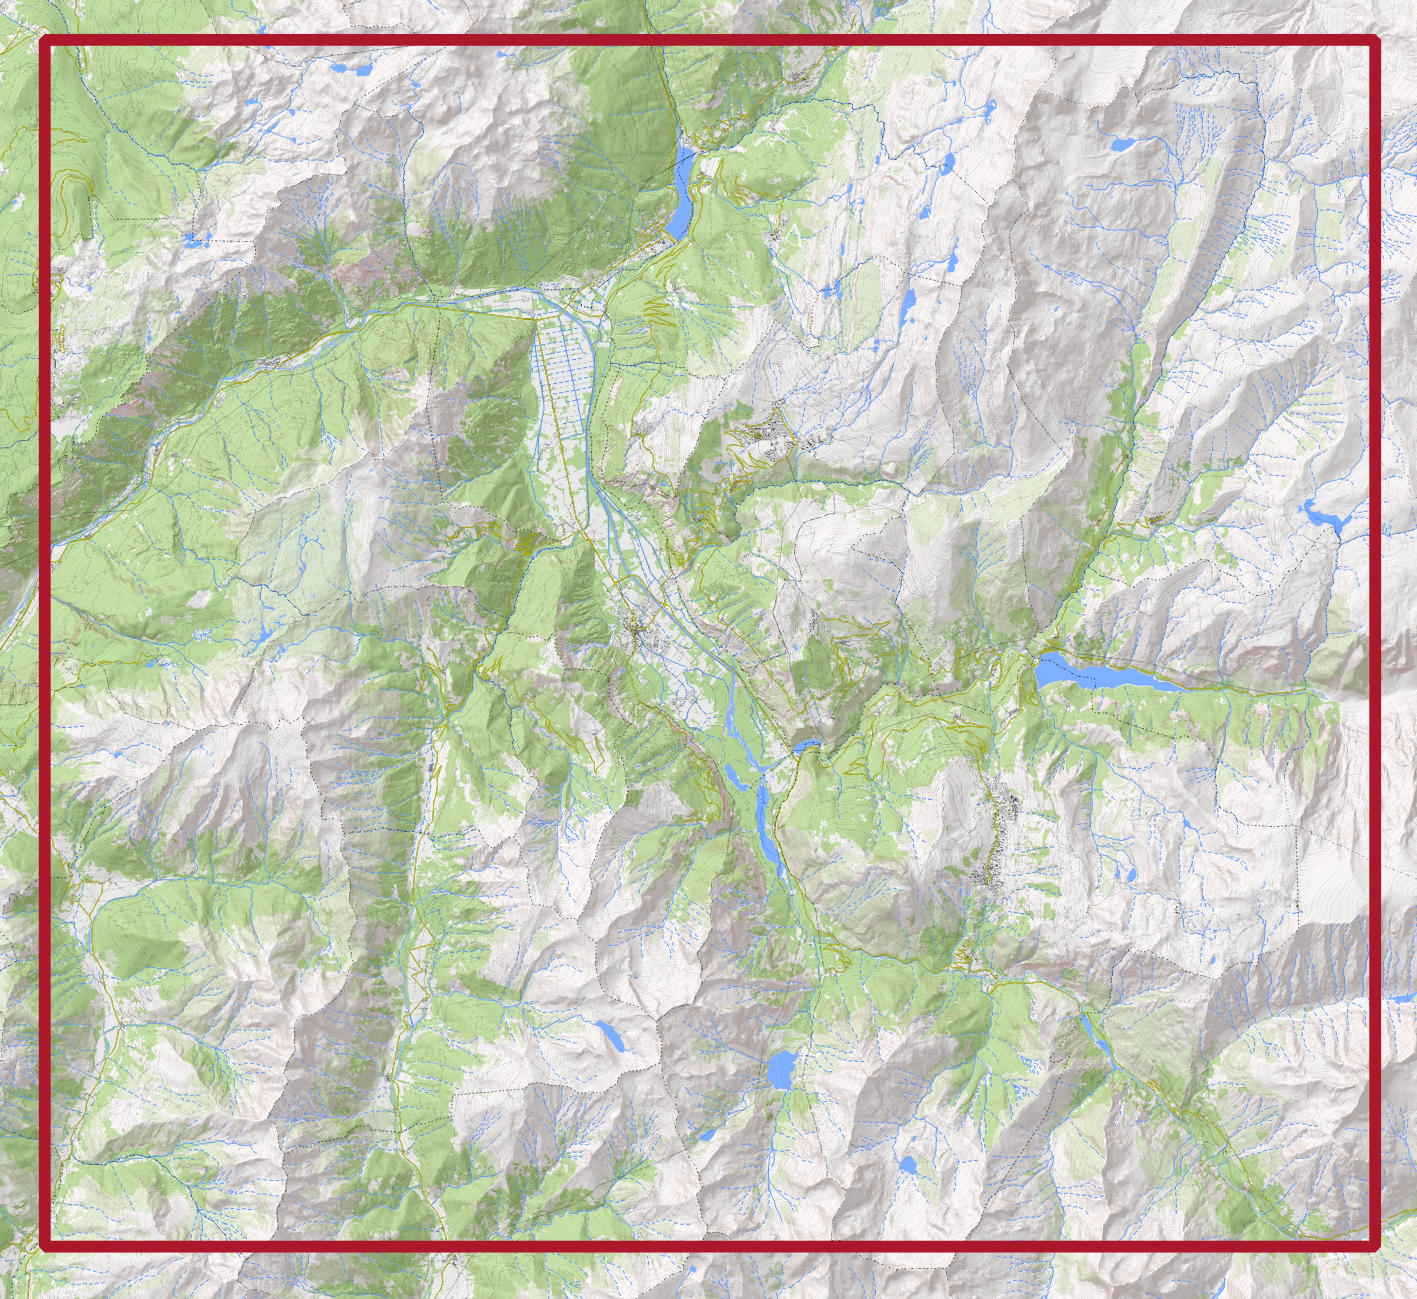
\includegraphics{./figures/ZIR_fil_rouge.png}};
  % 
  \begin{scope}
    \node (P2) at ([yshift=-.5cm]image.south east) {};
    \node (P1) at ([yshift=-.5cm]image.south west) {};
    % 
    \node (rect) [anchor=north west, minimum width=1cm,minimum
    height=.25cm] at ([yshift=-.25cm]P1) {}; \path[draw=RdBu-9-1, line
    width=1mm](rect.west) --([xshift=-1ex]rect.south) -- ([xshift=1ex]rect.north)
    -- (rect.east);
    % 
    \node[anchor=west, font=\tiny\vphantom{Ag}, text width = 4cm] at
    ([xshift=1ex]rect.east) {Limite de la \ac{zir}};
    % Échelle
    % Échelle
    \draw[-] (P2 |- -1cm,-1cm) --++ (-1,0) node[et,pos=.5] {\SI{2}{\kilo\meter}};
    % Légende détaillée
    \path (P1) -- (P2) node[pos=.5, yshift=-1cm] {\tiny Pour la légende détaillée du fond topographique voir \autoref{anx:topo_leg}. Sources: BD TOPO 2018, BD ALTI 2018.}; 
  \end{scope}
\end{tikzpicture}
  \caption{Zone initiale de recherche pour le \emph{fil rouge}}
  \label{fig:zir_fil_rouge}
\end{figure}

\subsubsection{Décomposition des indices de localisation}
\label{subsec:9-4-2-1}

\subsubsection{Spatialisation des indices de localisation}
\label{subsec:9-4-2-2}

\subsubsection{Fusion des zones de localisation compatibles}
\label{subsec:9-4-2-3}

\subsection{Critique de la modélisation}
\label{subsec:9-4-3}

\addsec{Conclusion / synthèse critique}

%%% Local Variables:
%%% mode: latex
%%% TeX-master: "../../../main"
%%% End:
